%%
\documentclass[format=draft,language=chinese,category=SDN]{hustreport}

\title{初赛文档}
\author{林家军~李英儒~胡云锐}
\major{计算机科学与技术}
\department{计算机科学与技术学院}
\advisor{周世伟}

\abstract{
    这是来自华中科技大学UniqueSDNStudio队伍的初赛文档,于\LaTeX{}编辑而成。

}
\keywords{软件定义网络, SDN, \LaTeX{}, 华中科技大学}


\begin{document}

\frontmatter
\maketitle
\makeabstract
\tableofcontents
\listoffigures
\listoftables
\mainmatter

\chapter{基础环境}\label{chapter:1}

\section{第一层}\label{sec:1}
\subsection{第二层}\label{sec:2}
\subsubsection{第三层}\label{sec:3}
测试测试测试测试测试测试测试测试测试测试测试测试。
\footnote{\label{footnote:1}脚注}

\section{字体}

普通\textbf{粗体}\emph{斜体}

\hei{黑体}\kai{楷体}\fangsong{仿宋}

\section{公式}

单个公式,公式引用:\autoref{eq:1}。
\begin{equation}
 c^2 = a^2 + b^2 \label{eq:1}
\end{equation}

多个公式,公式引用:\autoref{eq:2},\autoref{eq:3}。

\begin{subequations}
\begin{equation}
  F = ma \label{eq:2}
\end{equation}
\begin{equation}
  E = mc^2 \label{eq:3}
\end{equation}
\end{subequations}

\section{罗列环境}

\begin{enumerate}
    \item 第一层\label{item:1}
    \item 第一层
    \begin{enumerate}
        \item 第二层\label{item:2}
        \item 第二层
        \begin{enumerate}
            \item 第三层\label{item:3}
            \item 第三层
        \end{enumerate}
    \end{enumerate}
\end{enumerate}

\begin{description}
    \item[解释环境]  解释内容
\end{description}

\chapter{其他格式测试}

\section{代码环境}

\begin{lstlisting}[language=python]
import os

def main():
    '''
    doc here
    '''
    print 'hello, world' # Abc
    print 'hello, 中文' # 中文
\end{lstlisting}

\section{定律证明环境}

\begin{definition}\label{def:1}
这是一个定义。
\end{definition}
\begin{proposition}\label{proposition:1}
这是一个命题。
\end{proposition}
\begin{axiom}\label{axiom:1}
这是一个公理。
\end{axiom}
\begin{lemma}\label{lemma:1}
这是一个引理。
\end{lemma}
\begin{theorem}\label{theorem:1}
这是一个定理。
\end{theorem}
\begin{proof}\label{proof:1}
这是一个证明。
\end{proof}

\section{算法环境}

\begin{algorithm}[H]
\SetAlgoLined
\KwData{this text}
\KwResult{how to write algorithm with \LaTeX2e }
initialization\;\label{alg_line:1}
\While{not at end of this document}{
read current\;
\eIf{understand}{
go to next section\;
current section becomes this one\;
}{
go back to the beginning of current section\;
}
}
\caption{How to write algorithms}\label{alg:1}
\end{algorithm}

\section{表格}
表格见\autoref{tab:1}。

\begin{table}[!h]
\centering
\caption{一个表格}\label{tab:1}
\begin{tabular}{|c|c|}
\hline
a & b \\
\hline
c & d \\
\hline
\end{tabular}
\end{table}
\section{图片}
图片见\autoref{fig:1}。图片格式支持eps,png,pdf等。多个图片见\autoref{fig:2},分开引用:\autoref{fig:2-1},\autoref{fig:2-2}。

\begin{figure}[!h]
\centering
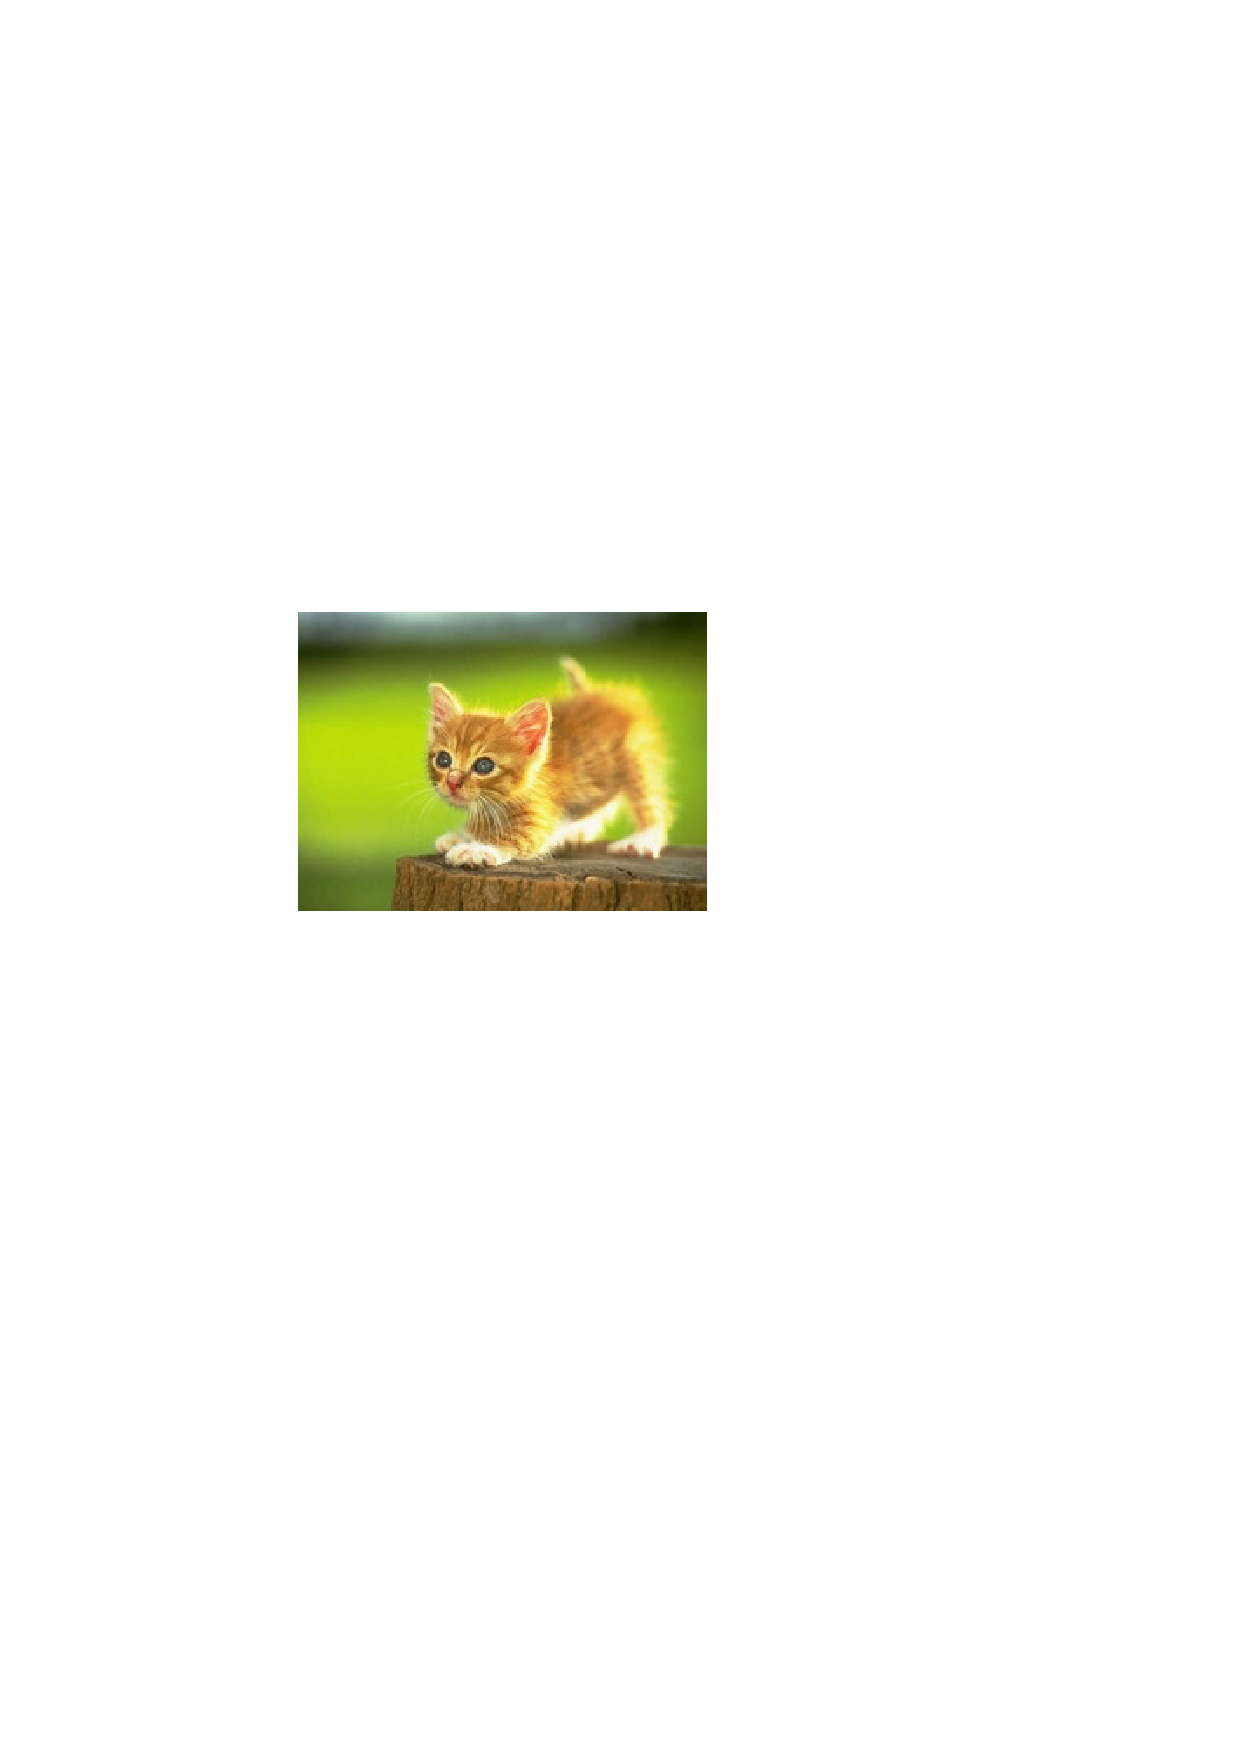
\includegraphics[width=.4\textwidth]{fig/fig-example.pdf}
\caption{一个图片}\label{fig:1}
\end{figure}

\begin{figure}[!h]
\centering
  \begin{subfigure}[b]{0.3\textwidth}
  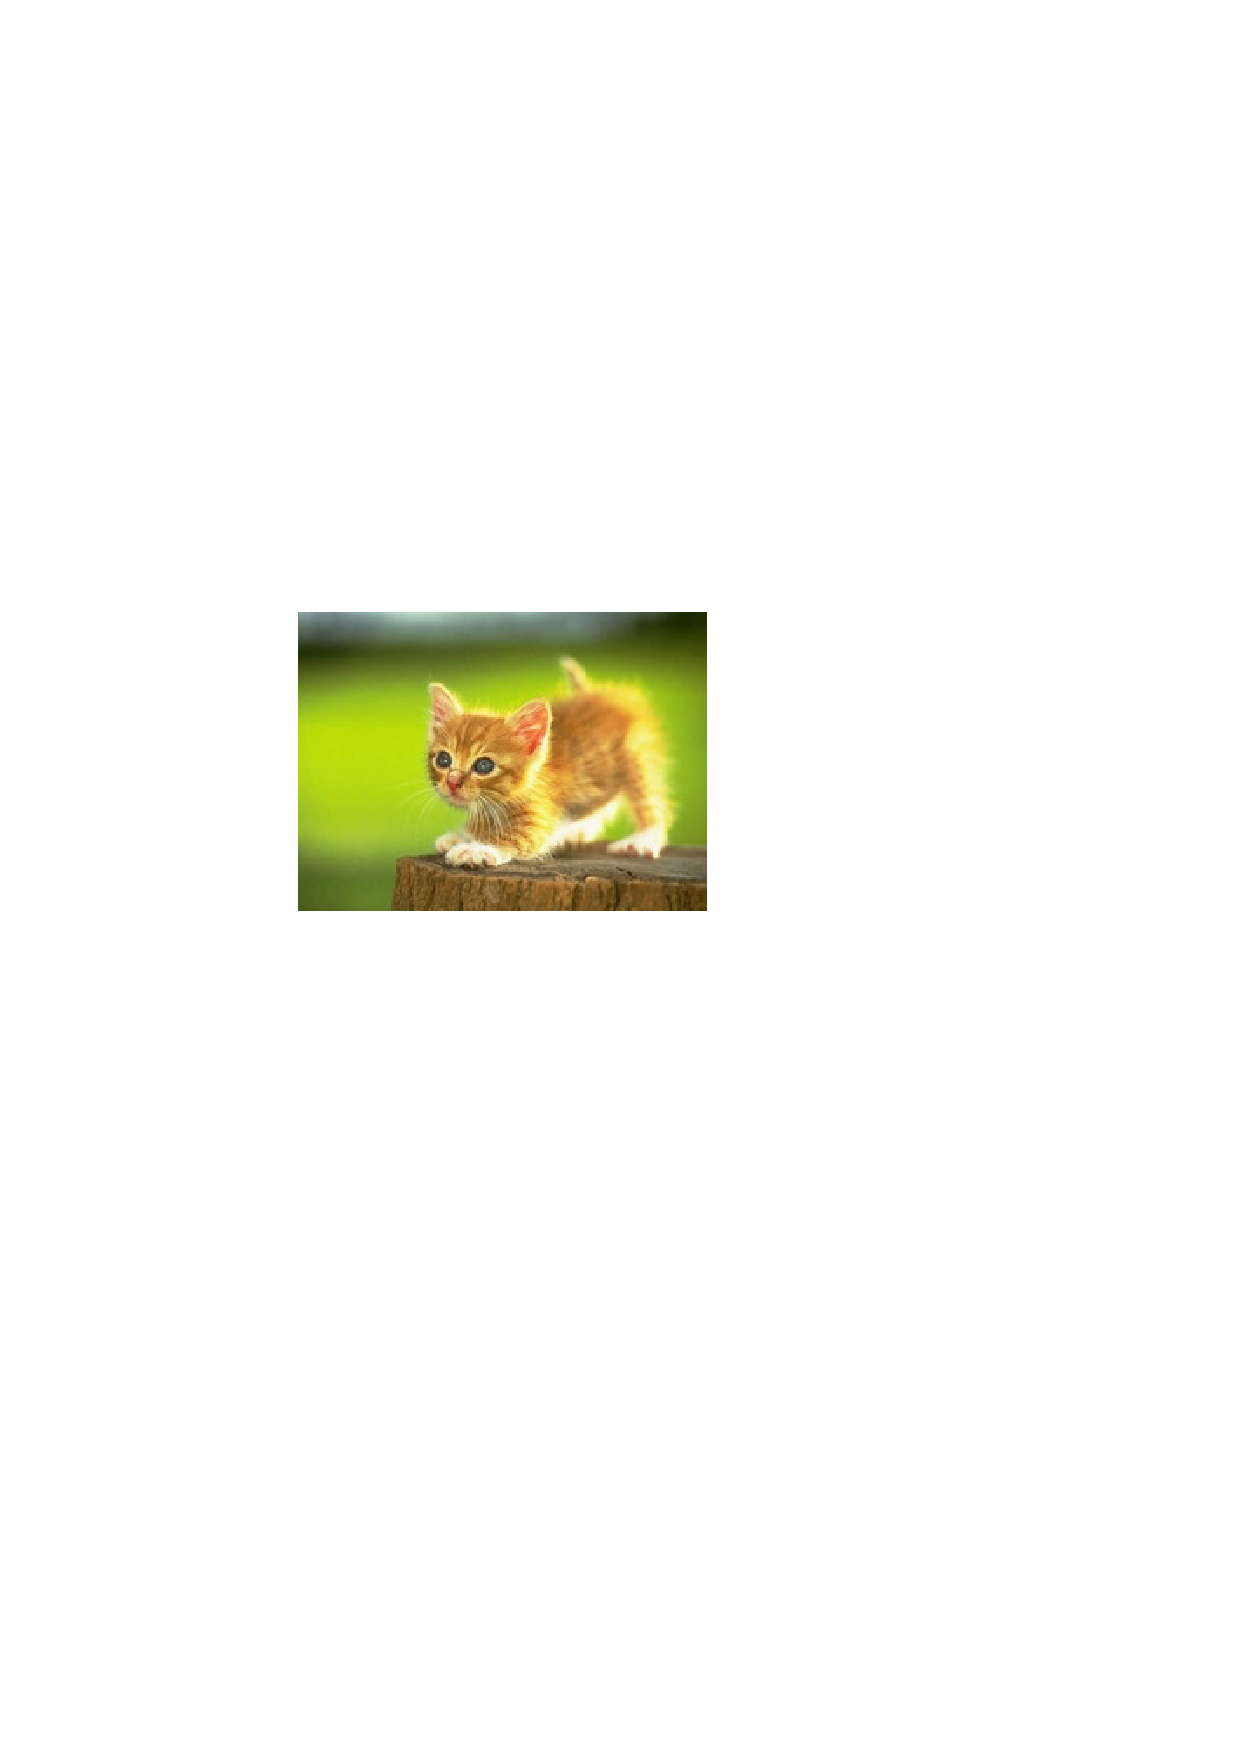
\includegraphics[width=\textwidth]{fig/fig-example.pdf}
  \caption{图片1}\label{fig:2-1}
  \end{subfigure}
  ~
  \begin{subfigure}[b]{0.3\textwidth}
  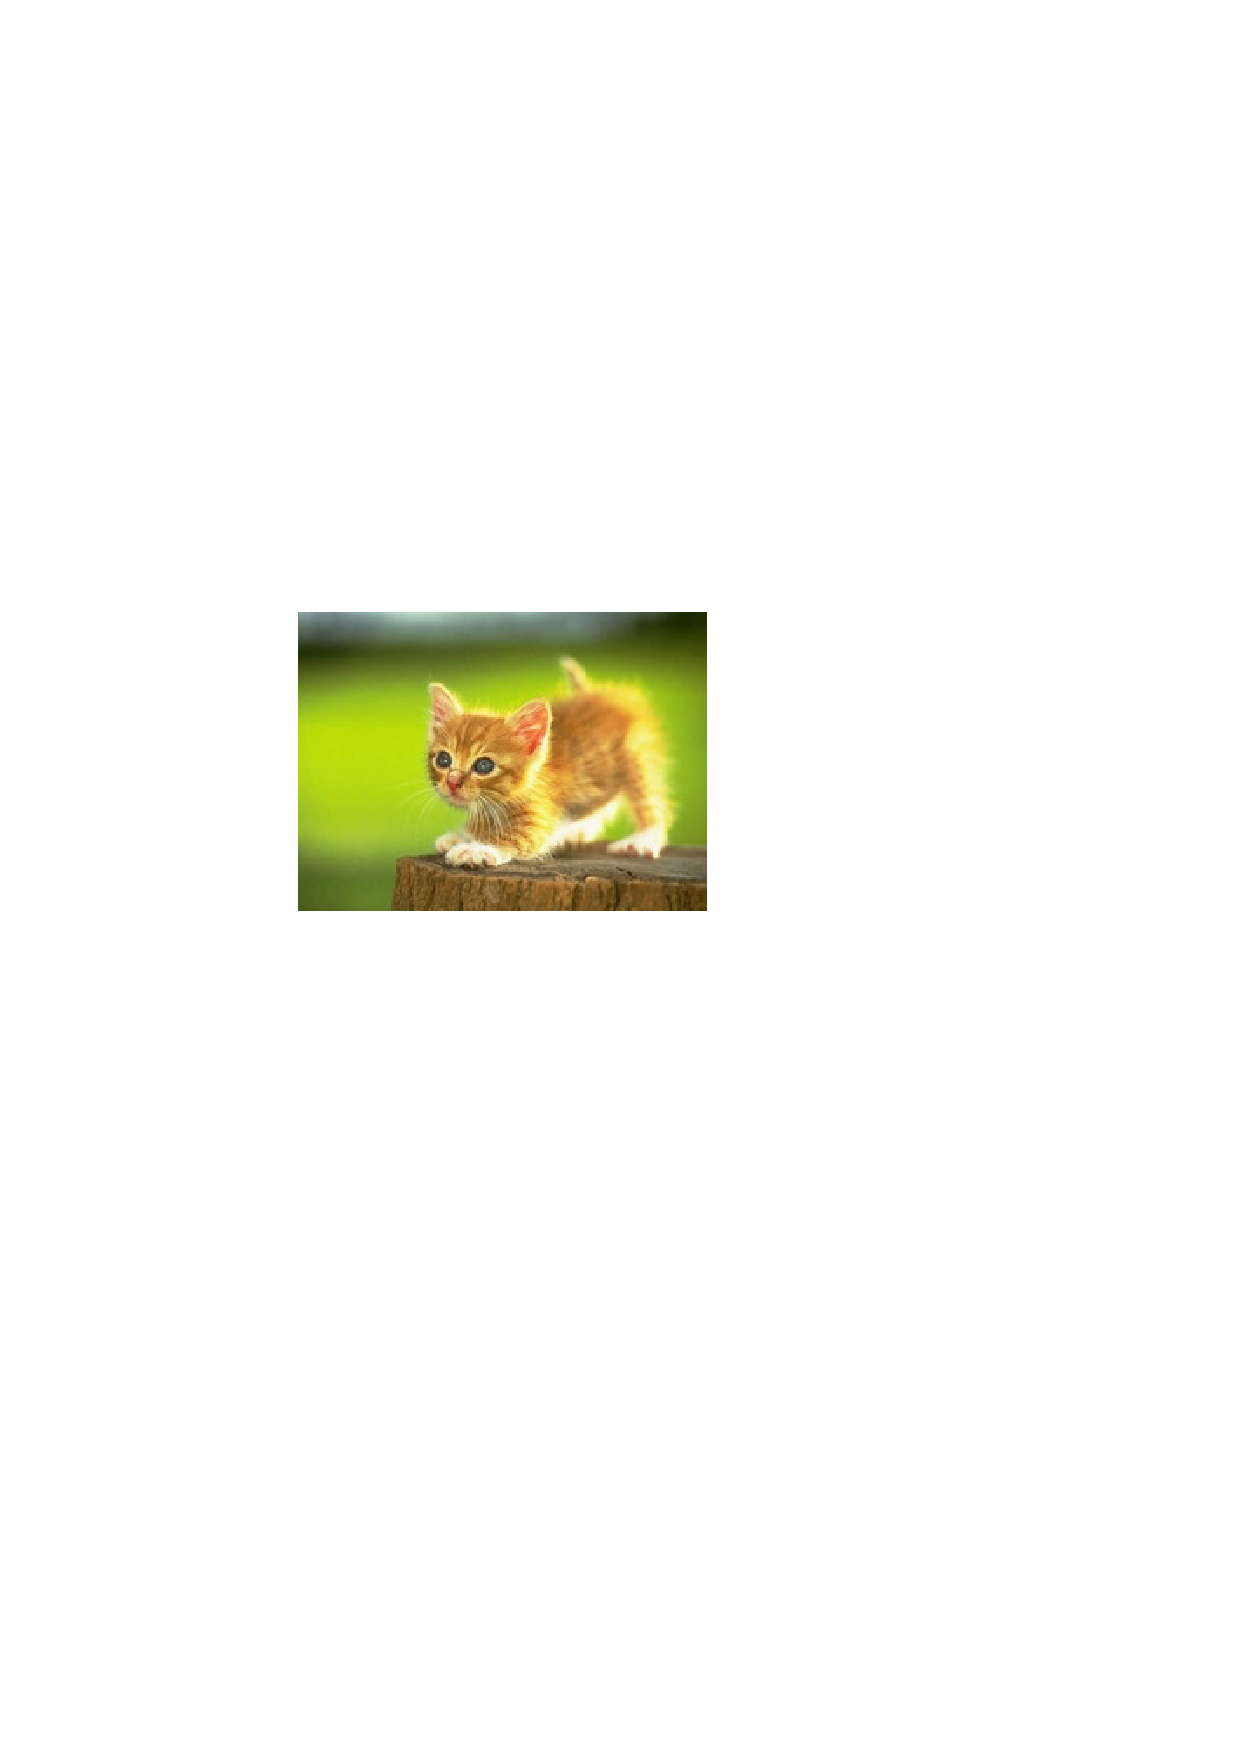
\includegraphics[width=\textwidth]{fig/fig-example.pdf}
  \caption{图片2}\label{fig:2-2}
  \end{subfigure}
\caption{多个图片}\label{fig:2}
\end{figure}

\section{参考文献示例}
这是一篇中文参考文献\cite{TEXGURU99};这是一篇英文参考文献\cite{knuth};同时引用\cite{TEXGURU99,knuth}。

\section[\textbackslash{}autoref 测试]{\texttt{\textbackslash{}autoref} 测试}

\begin{description}
  \item[公式] \autoref{eq:1}
  \item[脚注] \autoref{footnote:1}
  \item[项] \autoref{item:1},\autoref{item:2},\autoref{item:3}
  \item[图] \autoref{fig:1}
  \item[表] \autoref{tab:1}
  \item[附录] \autoref{appendix:1}
  \item[章] \autoref{chapter:1}
  \item[小节] \autoref{sec:1},\autoref{sec:2},\autoref{sec:3}
  \item[算法] \autoref{alg:1},\autoref{alg_line:1}
  \item[证明环境] \autoref{def:1},\autoref{proposition:1},\autoref{axiom:1},\autoref{lemma:1},\autoref{theorem:1},\autoref{proof:1}
\end{description}

\backmatter

\begin{ack}
致谢正文。
\end{ack}

\bibliography{ref-example}

\appendix

\begin{publications}
    \item 论文1
    \item 论文2
\end{publications}

\chapter{这是一个附录}\label{appendix:1}
附录正文。


\end{document}
\endinput
%%
%% End of file `hustreport-zh-example.tex'.
